\section{Mockups}
Com o propósito de criar um \textit{design} para seguir e apresentar às partes interessadas antes de iniciar a fase de desenvolvimento, então foram realizadas \textit{mockups} do \textit{design} da aplicação. Este \textit{design} foi iterativamente revisto pelo cliente e ajustado até alcançar o estado final.

\subsection{Página Inicial}

A página inicial da aplicação, dá ao utilizador a possibilidade de navegar pelos produtos do catálogo, filtrar por categorias e subcategorias, assim como realizar uma pesquisa rápida e por fim navegar para o fórum. Caso um técnico esteja com sessão iniciada este poderá visualizar o \textit{icon} de notificações e a sua imagem de perfil.

\begin{figure}[htb]
    \centering
    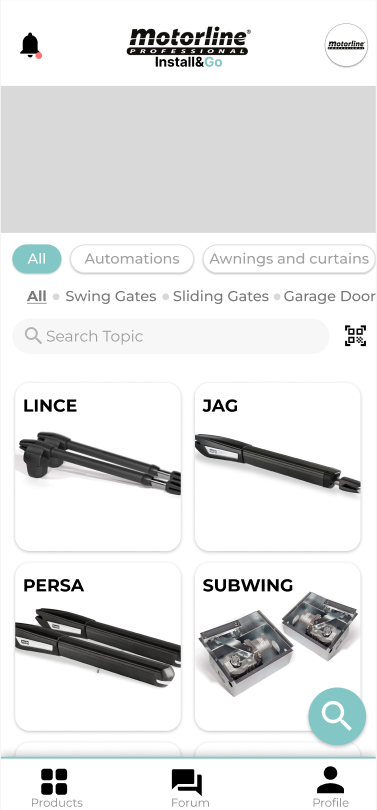
\includegraphics[width=0.45\textwidth]{images/mockups/home_screen.png}
    \caption{Página inicial do fórum}
    \label{fig:23}
\end{figure}

\newpage

\subsection{Autenticação - Login e Registo}

Na autenticação, é possível iniciar sessão e registo, mas a empresa é a única entidade poderá realizar o registo no \textit{software}.

\begin{figure}[htb]%
    \centering
    \subfloat[\centering Página de login]{{
\includegraphics[width=0.4\textwidth]{images/mockups/login.png} }}%
    \qquad
    \subfloat[\centering Página de registo]{{
\includegraphics[width=0.4\textwidth]{images/mockups/register.png} }}%
    \caption{Autenticação - Login e Registo}%
    \label{fig:24}
\end{figure}

\newpage

\subsection{Autenticação - Ativação e Confirmação de conta}

Na autenticação também existe a página de confirmação de conta. Um técnico que tem a conta recentemente adicionada poderá confirmar o registo, indicar as informações finais e por fim será direcionado para a página de ativação onde terá de colocar o código de ativação enviado para o \textit{email}, esta página também será aberta caso um técnico realize o \textit{login} com uma conta que não foi ativada ou sempre que um registo é finalizado.

\begin{figure}[htb]%
    \centering
    \subfloat[\centering Página de confirmação de conta]{{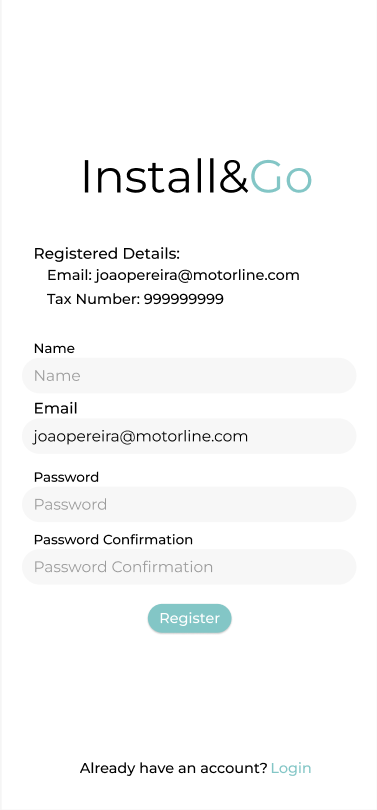
\includegraphics[width=0.4\textwidth]{images/mockups/account_confirmation.png} }}%
    \qquad
    \subfloat[\centering Página de ativação de conta]{{
\includegraphics[width=0.4\textwidth]{images/mockups/account_verification.png} }}%
    \caption{Autenticação - Ativação e Confirmação de conta}%
    \label{fig:25}%
\end{figure}

\newpage

\subsection{Página inicial fórum}

O técnico assim que se dirige ao fórum entrará na página inicial. Esta página permite navegar entre as diferentes listagens de tópicos acessíveis ao técnico, pesquisar, filtrar por tipo e criar um novo tópico.

\begin{figure}[htb]
    \centering
    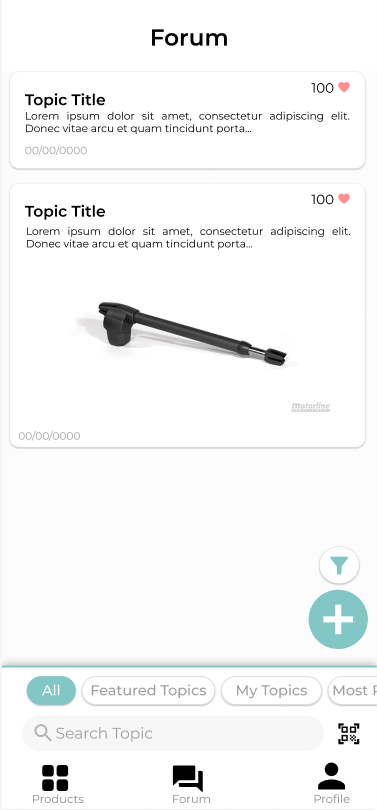
\includegraphics[width=0.45\textwidth]{images/mockups/forum_home.png}
    \caption{Página inicial do fórum}
    \label{fig:26}
\end{figure}

\newpage

\subsection{Página de detalhes de um tópico}

Assim que o técnico seleciona um tópico, será encaminhado para a página de detalhes, onde é indicado o nome do proprietário, a imagem de perfil, a hora de criação, a quantidade de gostos, o título, a descrição, as imagens e os comentários. É possível gostar do tópico, gostar de comentários, comentar o tópico e outros comentários.

Se o tópico for do técnico que está a visualizar, poderá também concluir, eliminar e alterar a sua visibilidade.

\begin{figure}[htb]%
    \centering
    \subfloat[\centering Página de detalhes de um tópico]{{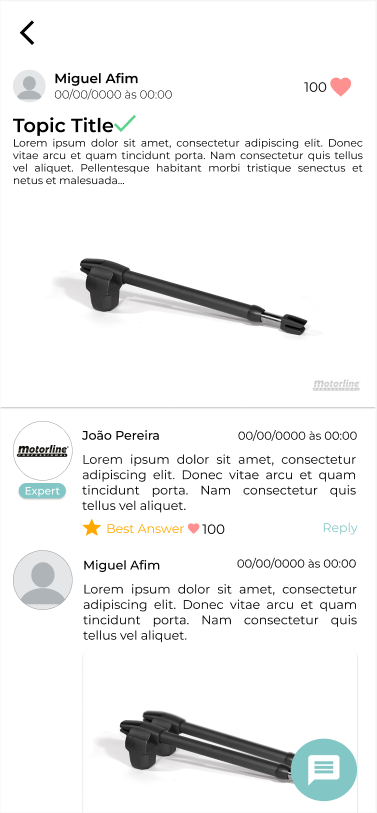
\includegraphics[width=0.4\textwidth]{images/mockups/topic_not_user.png} }}%
    \qquad
    \subfloat[\centering Página de detalhes de um tópico do técnico]{{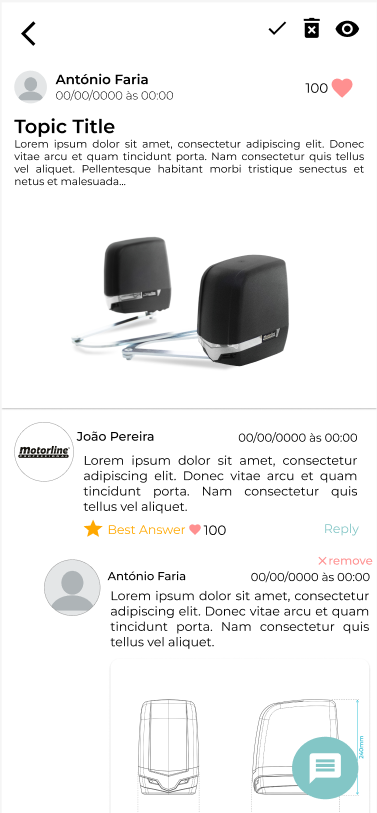
\includegraphics[width=0.4\textwidth]{images/mockups/user_topic.png} }}%
    \caption{Página de detalhes de tópico do software}%
    \label{fig:27}%
\end{figure}

\newpage

\subsection{Página de criação de um tópico}

Quando um técnico inicia a criação de um tópico, é obrigado a inserir o título e a descrição. Já a indicação da visibilidade, do tipo de tópico, do produto referente e de imagens é opcional. A qualquer momento poderá cancelar ou confirmar a ação.

\begin{figure}[htb]
    \centering
    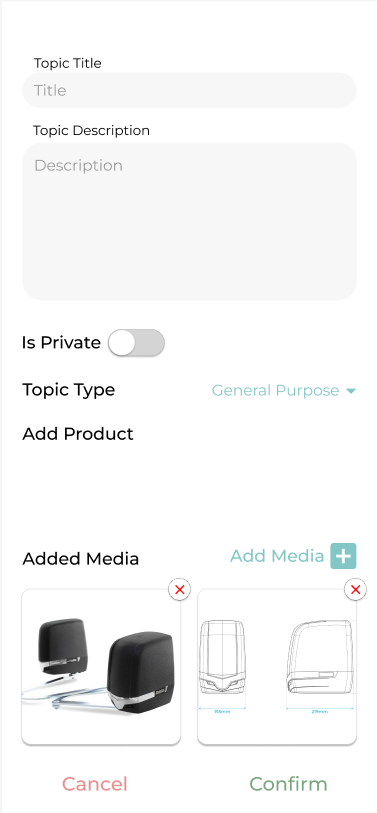
\includegraphics[width=0.45\textwidth]{images/mockups/forum_create_topic.png}
    \caption{Página de criação de tópico}
    \label{fig:28}
\end{figure}

\newpage

\subsection{Página de notificações}

Um técnico sempre que desejar tem como opção visualizar as suas notificações. Neste ecrã, é possível ver todas com a identificação de quem enviou, qual a descrição e a data de receção. O técnico, também tem como escolha apagar se assim desejar.

\begin{figure}[htb]
    \centering
    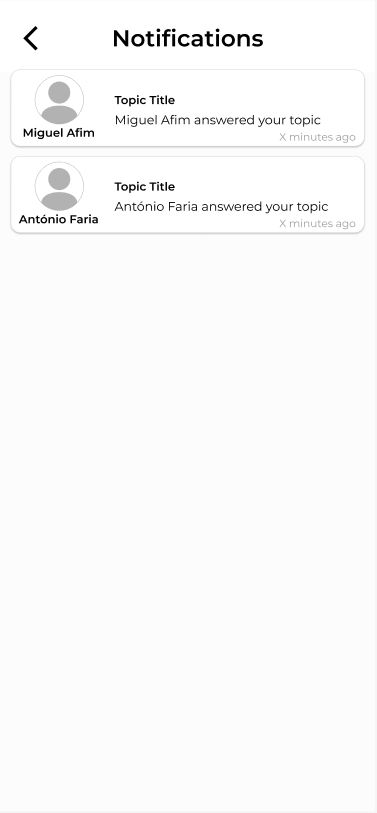
\includegraphics[width=0.45\textwidth]{images/mockups/notifications.png}
    \caption{Página de notificações}
    \label{fig:29}
\end{figure}

\newpage

\subsection{Página de perfil de utilizador}

O técnico, sempre que desejar alterar as suas informações, tem a possibilidade de modificar o \textit{email}, a imagem de perfil e a configuração das notificações com indicação dos métodos e tipo a receber.

Caso uma empresa entre no perfil, esta visualizará um botão para aceder à gestão de recursos humanos.

\begin{figure}[htb]
    \centering
    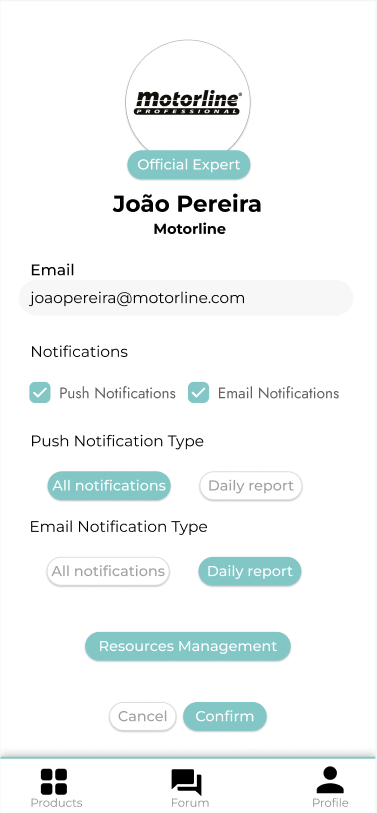
\includegraphics[width=0.45\textwidth]{images/mockups/user_profile.png}
    \caption{Página de perfil de utilizador}
    \label{fig:30}
\end{figure}

\newpage

\subsection{Página de gestão de recursos humanos}

Na página de gestão de recursos humanos, apenas acessível a empresas, é possível registar novos técnicos, pesquisar e gerir os que já se encontram registados através dos seus perfis.

\begin{figure}[htb]
    \centering
    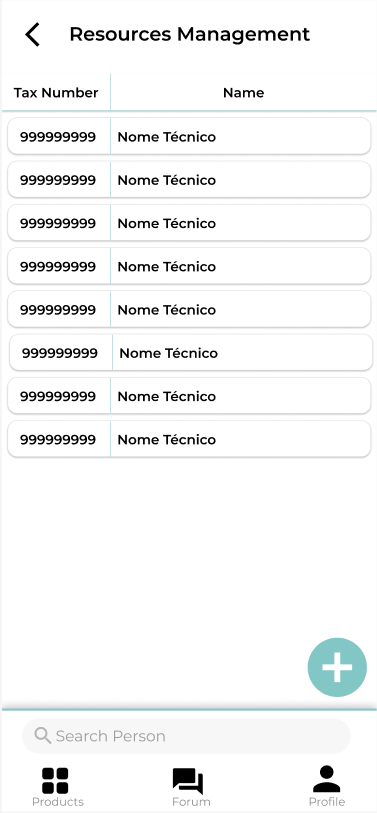
\includegraphics[width=0.45\textwidth]{images/mockups/human_resources.png}
    \caption{Página de gestão de recursos humanos}
    \label{fig:31}
\end{figure}

\newpage

\subsection{Página de perfil de técnico registado}

O perfil de técnico, apenas acessível para empresas, permite visualizar as estatísticas, as informações e permite impedir acesso à conta ou então remover da plataforma.

\begin{figure}[htb]
    \centering
    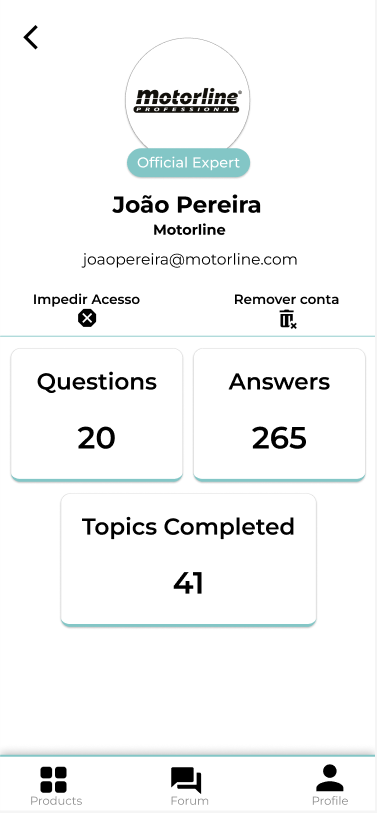
\includegraphics[width=0.45\textwidth]{images/mockups/professional_profile.png}
    \caption{Página de perfil de técnico registado}
    \label{fig:32}
\end{figure}

\newpage

\subsection{Página de registo de novo técnico}

Sempre que uma empresa deseja registar um novo técnico, esta deverá indicar o nome, o \textit{email} e tipo de técnico.

\begin{figure}[htb]
    \centering
    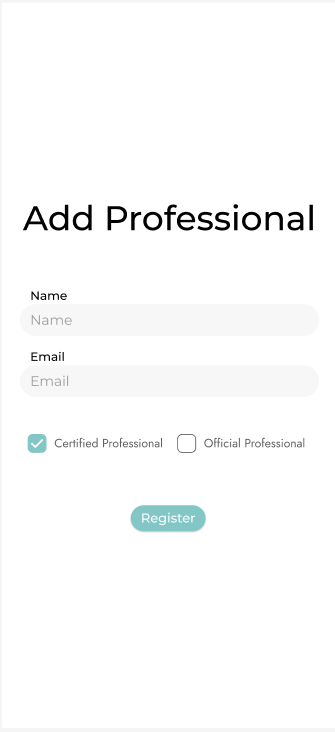
\includegraphics[width=0.45\textwidth]{images/mockups/account_registering.png}
    \caption{Página de registo de novo técnico}
    \label{fig:33}
\end{figure}